\documentclass[10pt,twocolumn,letterpaper]{article}

\usepackage{cvpr}
\usepackage{times}
\usepackage{epsfig}
\usepackage{graphicx}
\usepackage{amsmath}
\usepackage{amssymb}
\usepackage{booktabs}
\usepackage{float}
\usepackage{placeins}
\usepackage[breaklinks=true,bookmarks=false]{hyperref}

\cvprfinalcopy

\def\cvprPaperID{****}
\def\httilde{\mbox{\tt\raisebox{-.5ex}{\symbol{126}}}}

\setcounter{page}{1}
\raggedbottom
\setlength{\textfloatsep}{6pt plus 1pt minus 2pt}
\setlength{\floatsep}{5pt plus 1pt minus 2pt}
\setlength{\intextsep}{5pt plus 1pt minus 2pt}

\begin{document}

\title{Multimodal Contradiction Detection on a COCO-Derived Benchmark: Comparing CLIP-Based Models and Qwen2.5-VL}

\author{Saj Patel, Prathamesh Swar\\
COMP 646, Rice University\\
{\tt\small [sp258, ps165]@rice.edu}
}

\maketitle

\begin{abstract}
Multimodal contradiction detection asks whether an image supports or conflicts with a caption, but common image-text datasets do not isolate contradiction types in a controlled way. We build a COCO-derived binary benchmark with 4,552 examples from 2,276 source families, balanced between entailment and contradiction and organized into action, attribute, object, and count edits with family-level train/validation/test splits. On the final 684-example comparison set, a cross-attention classifier over frozen OpenAI CLIP ViT-B/32 token states reaches 96.5\% accuracy, outperforming a frozen CLIP linear probe (89.6\%), raw CLIP thresholding (62.6\%), and zero-shot Qwen2.5-VL-3B-Instruct (76.3\%). The largest gap appears on count edits, suggesting that supervised fusion over strong frozen vision-language features is more reliable than raw similarity or zero-shot prompting for structured contradiction detection.
\end{abstract}
\vspace{-0.6em}

\section{Introduction}
\noindent
Modern vision-language models are strong on image-text retrieval and caption-aligned matching~\cite{radford2021learning}, but those capabilities do not guarantee reliable visual grounding when a caption conflicts with the image. Multimodal contradiction detection is stricter: the model must decide whether a caption is actually supported by the image rather than merely related to it.

Existing benchmarks do not isolate contradiction types in a compact, controlled way. Microsoft COCO~\cite{lin2014microsoft} provides broad visual coverage, but it is not designed for structured contradiction analysis. We therefore build a COCO-derived benchmark from \texttt{val2017} captions, apply meaning-preserving synonym edits for entailment, introduce targeted contradiction edits, and split data at the source-family level to prevent leakage across train, validation, and test. This lets us compare raw similarity, frozen-feature classification, token-level multimodal fusion, and zero-shot prompting under matched contradiction families.

\section{Related Work}
\noindent
FOIL-COCO shows that controlled caption edits expose failures in image-language grounding~\cite{shekhar2017foil}. SNLI-VE studies visual entailment over image-sentence pairs and motivates evaluation beyond captioning or question answering~\cite{xie2019visual}. NLVR2 frames a related truth-evaluation problem over paired photographs and human-written statements, with examples involving quantities, comparisons, and relations~\cite{suhr2019nlvr2}. These datasets motivate our binary formulation, but our benchmark keeps the edit operation explicit so each contradiction has a known source caption and edit family.

Recent compositionality benchmarks also show that high retrieval or captioning performance does not imply fine-grained grounding. Winoground tests whether models match reordered captions to images when the captions contain the same words~\cite{thrush2022winoground}. ARO evaluates attribution, relation, and word-order sensitivity and finds that standard vision-language models often behave like bag-of-words matchers~\cite{yuksekgonul2023bags}. VALSE evaluates linguistic phenomena through valid foils, while SugarCrepe argues that compositional benchmarks need hard negatives that reduce exploitable dataset bias~\cite{parcalabescu2022valse,hsieh2023sugarcrepe}. Our benchmark is narrower than these broad suites, but it gives a simple controlled testbed for action, attribute, object, and count contradictions.

The work also connects to recent evaluation of hallucination in large vision-language models. POPE probes whether such models mention objects that are not present in the image~\cite{li2023pope}. Our task is complementary: instead of evaluating free-form generations, the benchmark asks whether a model rejects a supplied caption when a targeted edit makes the caption false. CLIP provides strong contrastive image-text representations and makes direct similarity thresholding a natural baseline~\cite{radford2021learning}. We compare that baseline with learned classifiers on frozen CLIP features and Qwen2.5-VL as a modern zero-shot reference~\cite{bai2025qwen}.

\section{Benchmark Construction}
\noindent
We build the benchmark from a subset of COCO 2017 \texttt{val2017} captions~\cite{lin2014microsoft}. A \textit{source family} contains one original caption and all edited captions derived from it. We retain a family only when it yields both an entailment edit and at least one contradiction edit, then split at the family level so near-duplicate caption variants never cross train, validation, and test.

The final benchmark contains 2,276 source families, 4,552 total examples, and 1,239 unique images. The resulting split is 3,186 training examples, 682 validation examples, and 684 test examples. Each family contributes one entailment example and one contradiction example. Entailment rows use meaning-preserving synonym edits such as \textit{people} $\rightarrow$ \textit{individuals} or \textit{couch} $\rightarrow$ \textit{sofa}. Contradiction rows use four rule families: action edits (for example \textit{sitting} $\rightarrow$ \textit{running}), attribute edits (\textit{blue} $\rightarrow$ \textit{red}), object edits (\textit{couch} $\rightarrow$ \textit{bench}), and count edits (\textit{two} $\rightarrow$ \textit{one}).

Before inclusion, edits are filtered for phrase integrity, grammatical agreement, and object replacements that already appear in the image metadata. Contradiction coverage is therefore intentionally uneven. The final benchmark contains 683 action contradictions, 642 count contradictions, 567 object contradictions, and 384 attribute contradictions. Figure~\ref{fig:benchmark_family_counts} summarizes the benchmark composition.

\begin{figure}[t]
\centering
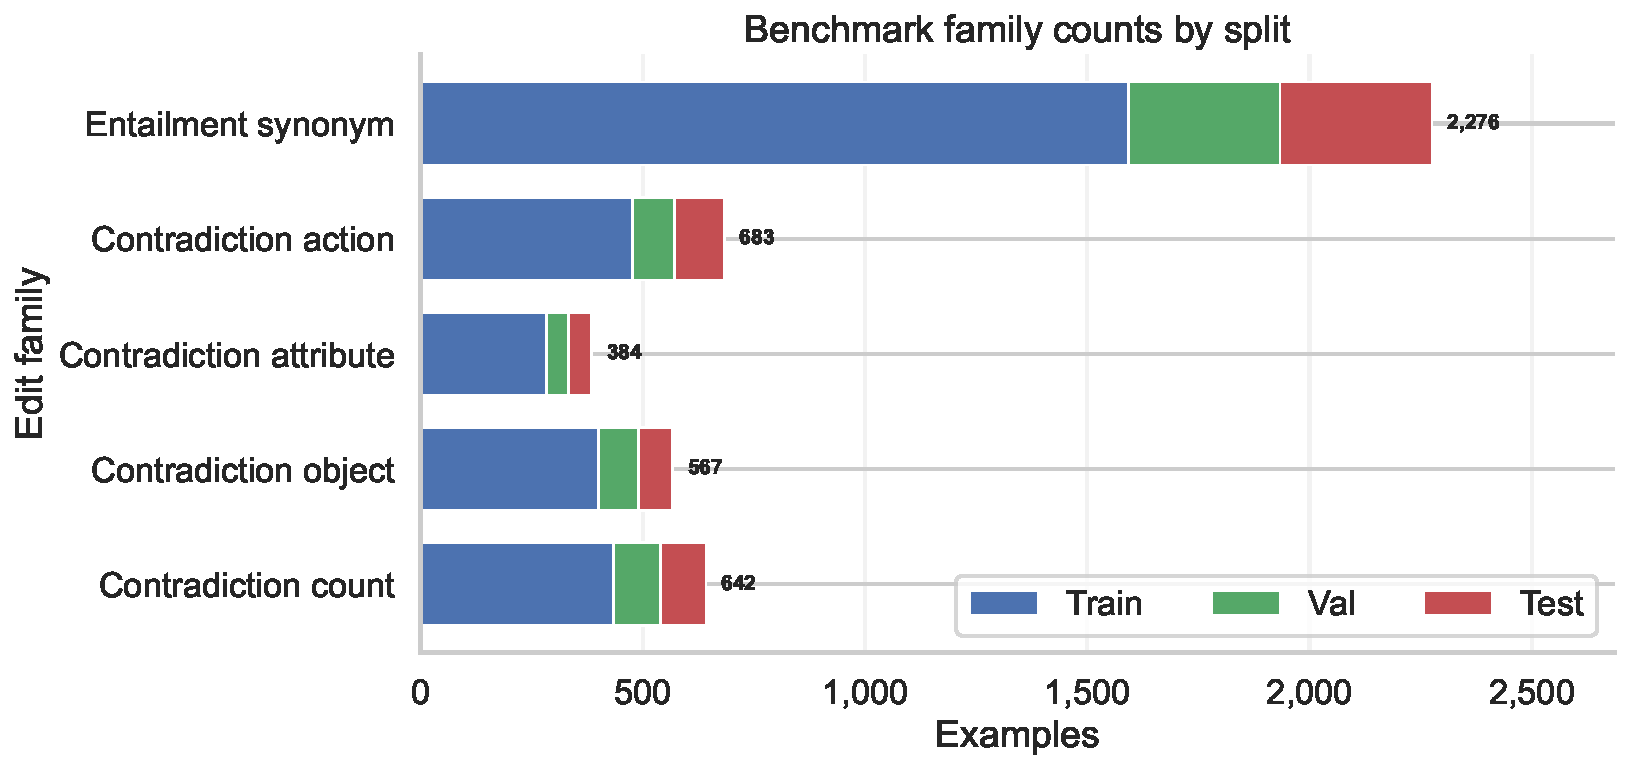
\includegraphics[width=\linewidth]{figures/generated/benchmark_family_counts_final.pdf}
\caption{Final benchmark composition. Stacked horizontal bars show example counts for each edit family, colored by split (train/validation/test), with totals shown at right. The benchmark is balanced overall between entailment and contradiction, but contradiction subfamilies remain uneven because some clean edits are easier to generate from COCO captions than others.}
\label{fig:benchmark_family_counts}
\end{figure}

\section{Models and Experimental Setup}
\noindent
We compare four systems built around two concrete pretrained checkpoints. The shared backbone for the first three systems is \textbf{OpenAI CLIP ViT-B/32} (`\texttt{openai/clip-vit-base-patch32}`), a dual-encoder model with about 151.3M parameters across its vision and text towers~\cite{radford2021learning}. Our zero-shot reference is \textbf{Qwen2.5-VL-3B-Instruct} (`\texttt{Qwen/Qwen2.5-VL-3B-Instruct}`), a 3.75B-parameter vision-language model according to the Hugging Face checkpoint metadata~\cite{bai2025qwen}. After these first mentions, we refer to them as CLIP and Qwen2.5-VL for brevity.

\textbf{Raw CLIP} uses CLIP ViT-B/32 to compute cosine similarity between normalized image and text embeddings, then predicts contradiction or entailment with a threshold fit on the validation set. This is a natural baseline, but cosine similarity is a retrieval score rather than a calibrated contradiction classifier. \textbf{Linear Probe} keeps the same CLIP backbone frozen and trains a classifier on the pooled image embedding, pooled text embedding, and raw CLIP score, testing whether frozen global features are already sufficient. \textbf{Cross-Attention} also keeps CLIP frozen, but replaces pooled-only features with token-level fusion: image and text token states are projected to hidden size 256, fused with 4-head cross-attention, mean pooled, and fed to a binary classifier. This adds explicit image-text interactions that should help on localized edits such as counts or attributes. \textbf{Qwen2.5-VL} is used zero-shot: it receives the image and edited caption and returns a JSON label indicating contradiction or entailment.

For the learned CLIP models, we train only the added classifier layers and keep the CLIP backbone frozen throughout. Validation sweeps select the best linear probe (30 epochs, batch size 16, learning rate $5\times10^{-4}$) and cross-attention model (35 epochs, batch size 4, learning rate $10^{-4}$). Raw CLIP uses the best validation threshold $\tau=0.2907$, and Figure~\ref{fig:raw_clip_threshold} shows the validation sweep that selects this operating point. The learned models also use validation-based early stopping so runs can terminate once accuracy plateaus instead of always consuming the full epoch budget. In the final run, all four systems are compared on the same 684-example evaluation set; this comparison set equals the full test split. We report overall accuracy, class-specific F1, and per-family accuracy by edit type.

\begin{figure}[t]
\centering
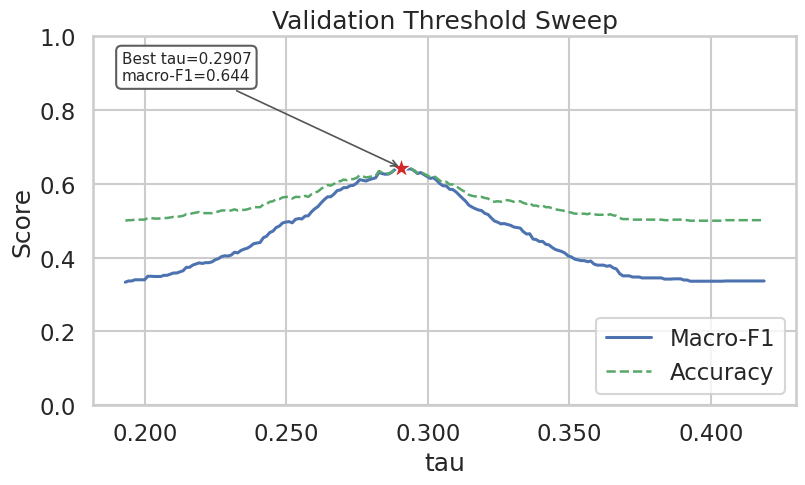
\includegraphics[width=\linewidth]{figures/generated/raw_clip_threshold_sweep_final.png}
\caption{Raw CLIP validation threshold sweep. The blue and dashed green curves show macro-F1 and accuracy as the contradiction threshold $\tau$ varies, and the star marks the selected validation threshold $\tau=0.2907$. This diagnostic shows that raw CLIP needs an explicit decision rule rather than relying on cosine similarity alone.}
\label{fig:raw_clip_threshold}
\end{figure}

\section{Results}
\noindent
Table~\ref{tab:main_results} shows the main quantitative comparison on the 684-example evaluation set. Raw CLIP similarity is a weak baseline on this task, while both learned CLIP-based classifiers improve sharply over thresholding alone. The cross-attention model is strongest overall at 96.5\% accuracy, followed by the linear probe at 89.6\%. Qwen2.5-VL is a useful zero-shot reference, but it remains well below the learned CLIP models on this controlled benchmark. Figure~\ref{fig:training_dynamics} adds an optimization view of the two learned CLIP models: under the same early-stopping procedure, the linear probe continues improving until epoch 25 and stops at epoch 27, while cross-attention peaks by epoch 8 and stops at epoch 10. This gap suggests that the token-level fusion model reaches a stable solution much earlier than the pooled-feature linear probe on this benchmark.

\begin{table}[H]
\centering
\scriptsize
\setlength{\tabcolsep}{3pt}
\begin{tabular}{@{}lccc@{}}
\toprule
\textbf{Model} & \textbf{Accuracy} & \textbf{Contradiction F1} & \textbf{Entailment F1} \\
\midrule
Raw CLIP & 0.626 & 0.619 & 0.632 \\
Linear Probe & 0.896 & 0.897 & 0.895 \\
Cross-Attention & 0.965 & 0.965 & 0.965 \\
Qwen2.5-VL & 0.763 & 0.709 & 0.800 \\
\bottomrule
\end{tabular}
\caption{Final comparison on the 684-example evaluation set. Accuracy is overall binary accuracy; Contradiction F1 and Entailment F1 are class-specific F1 scores. Higher is better.}
\label{tab:main_results}
\end{table}

\begin{figure}[t]
\centering
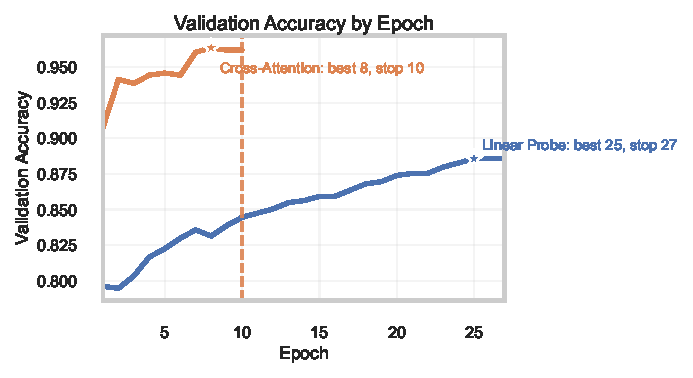
\includegraphics[width=\linewidth]{figures/generated/training_dynamics_final.pdf}
\caption{Validation-accuracy traces for the selected learned CLIP models. Stars mark the best validation epoch retained for checkpoint selection, and dashed lines mark the stop epoch under early stopping. The linear probe stopped after 27 epochs, while cross-attention stopped after 10.}
\label{fig:training_dynamics}
\end{figure}

Figure~\ref{fig:per_family_heatmap} breaks accuracy down by edit family. The cross-attention model remains strongest across every family, while the linear probe loses more accuracy on attribute edits. Count contradictions are the clearest stress test: they require exact visual grounding rather than coarse semantic similarity, and this is where Qwen is least stable. Figure~\ref{fig:qualitative_results} expands the qualitative analysis to eight unique examples: four contradiction cases on the top row and four entailment synonym cases on the bottom row, with each panel showing the original image, the full source caption, the edited caption, and a matched pair of model predictions.

\begin{figure}[t]
\centering
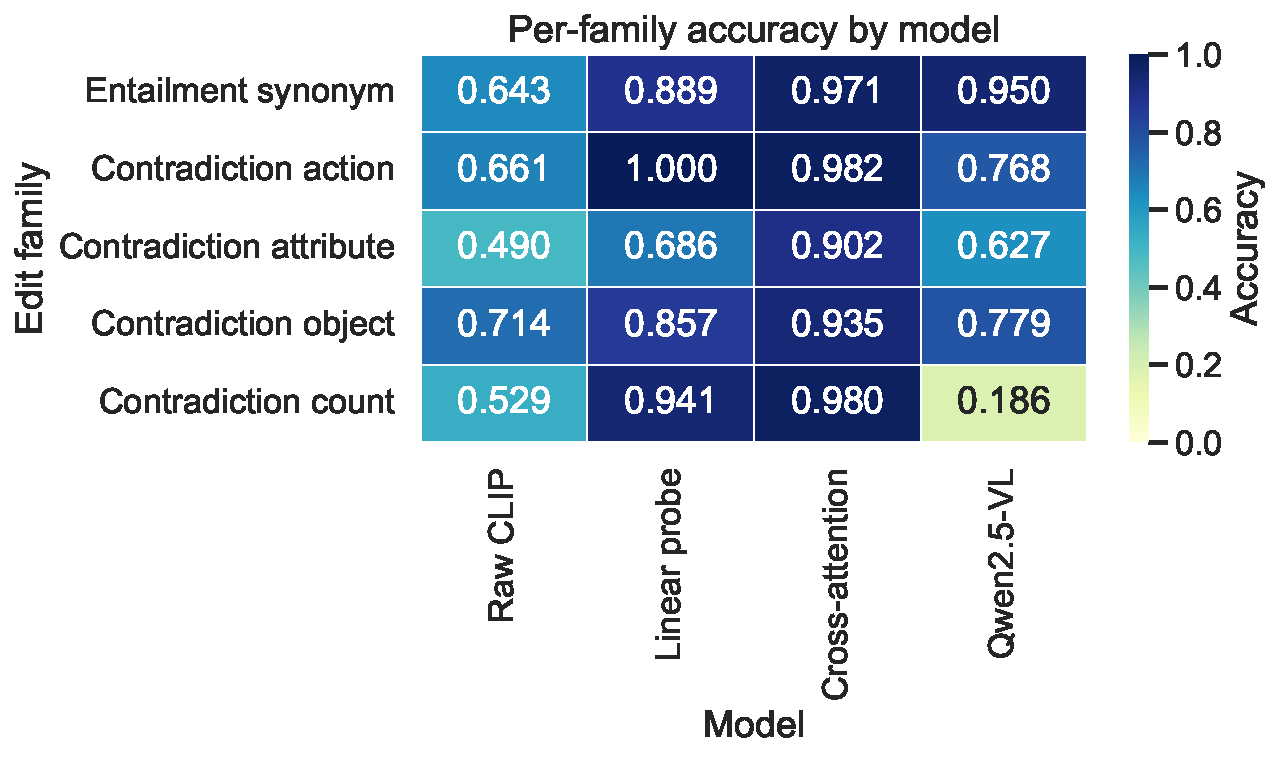
\includegraphics[width=\linewidth]{figures/generated/model_comparison_per_family_accuracy_final.pdf}
\caption{Per-family accuracy on the final 684-example evaluation set. Count edits are the hardest family for the zero-shot Qwen baseline, while cross-attention remains strong across all edit types.}
\label{fig:per_family_heatmap}
\end{figure}

\begin{figure*}[!t]
\centering
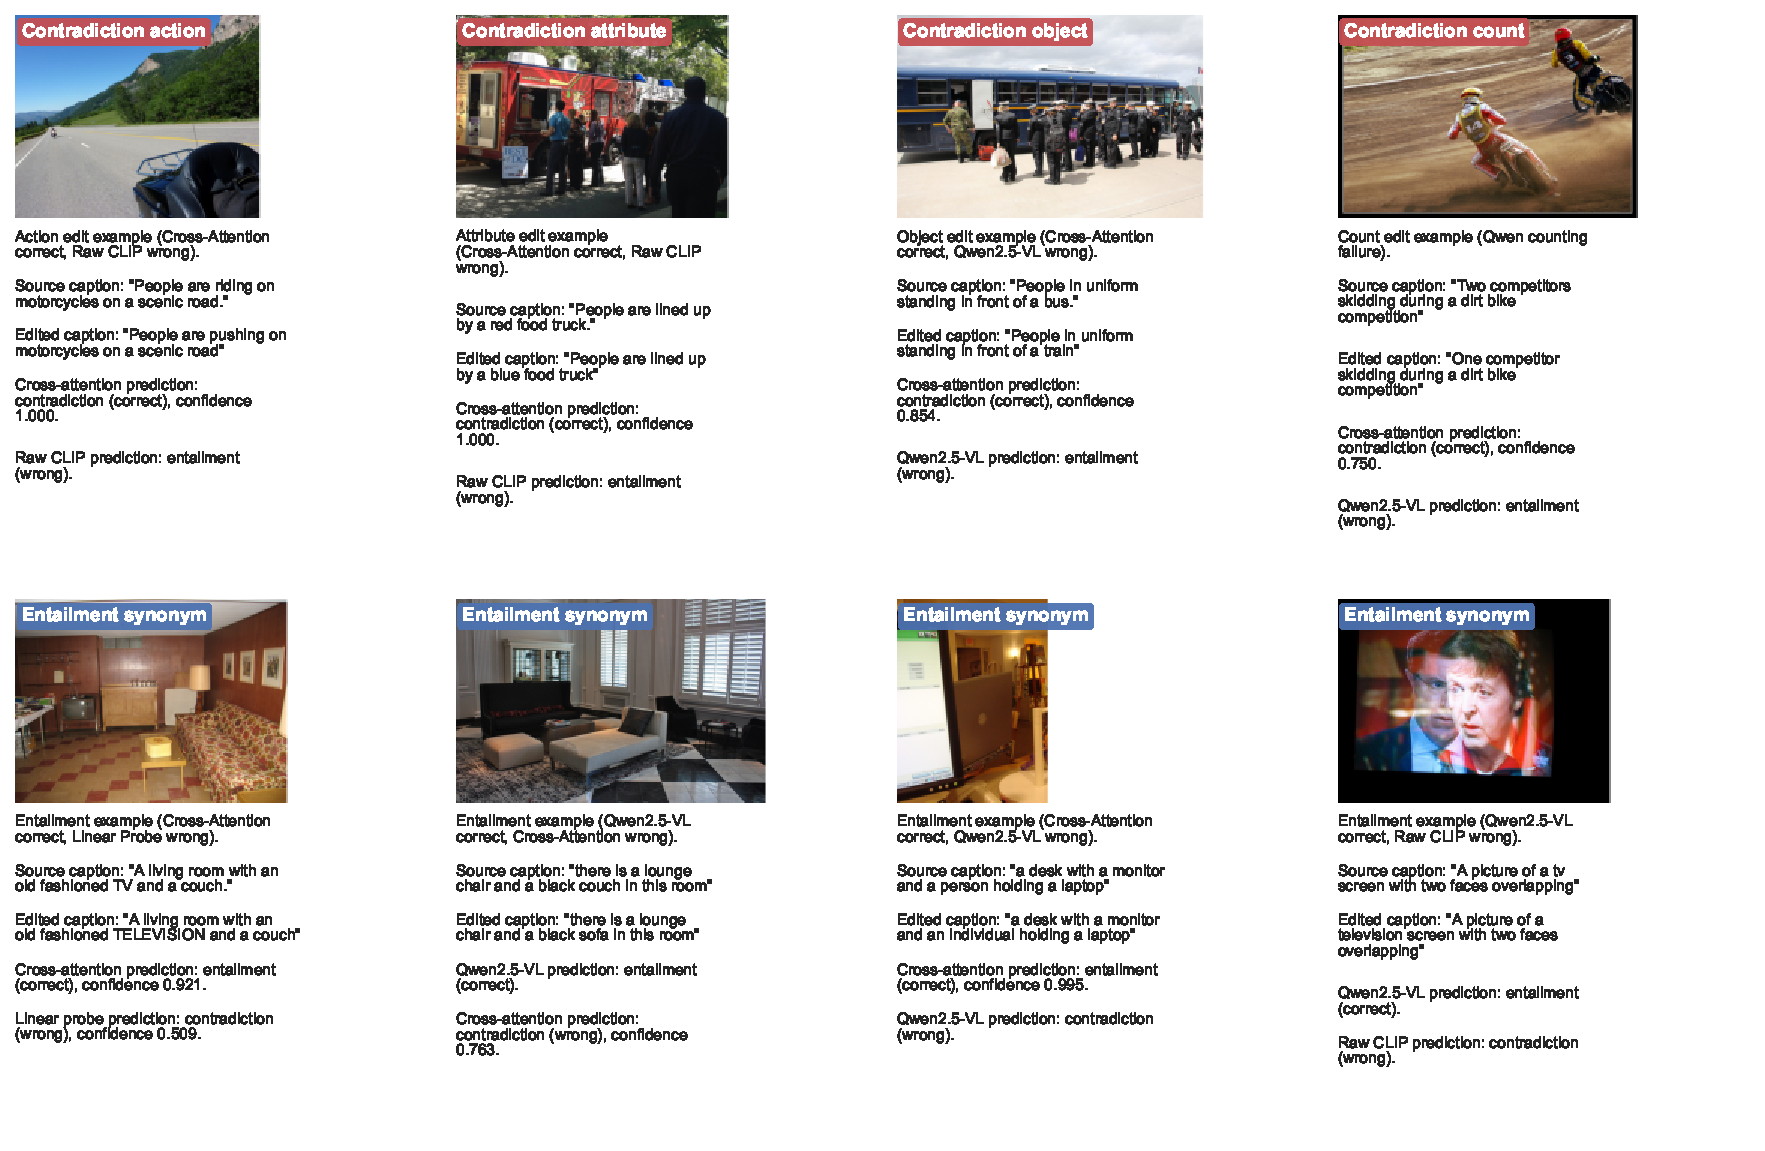
\includegraphics[width=\textwidth]{figures/generated/qualitative_gallery_final.pdf}
\caption{Qualitative model behavior on eight test examples. The top row shows contradiction edits and the bottom row shows entailment synonym edits. Each panel includes the image, source caption, edited caption, and paired model predictions; Cross-Attention is strongest overall, while Qwen fails most clearly on count edits.}
\label{fig:qualitative_results}
\end{figure*}

\paragraph{Error Analysis.}
The strongest separation appears on count contradictions. In Figure~\ref{fig:per_family_heatmap}, each cell reports per-family accuracy for one model-family pair. The count row shows the widest spread: Cross-Attention reaches 0.980 accuracy, compared with 0.941 for the linear probe, 0.529 for raw CLIP, and only 0.186 for Qwen. Qwen's overall accuracy remains higher than raw CLIP because it is strong on entailment synonyms (0.950), but it often treats number edits as semantically compatible with the image, as Figure~\ref{fig:qualitative_results} illustrates. Attribute edits are the second clearest separator in Figure~\ref{fig:per_family_heatmap}: Cross-Attention reaches 0.902 accuracy, while the linear probe drops to 0.686, Qwen to 0.627, and raw CLIP to 0.490.

A second pattern is class bias. Qwen's contradiction recall is 0.576 overall, far below its entailment recall of 0.950, suggesting that the zero-shot model often accepts edited captions unless the mismatch is unmistakable. Cross-attention remains balanced across classes (0.965 F1 for contradiction and 0.965 F1 for entailment), which is important because the core error in this task is falsely accepting incorrect captions.

\section{Discussion}
\noindent
The main technical result is that structured contradiction detection benefits from supervised fusion over frozen CLIP features, not just larger zero-shot model scale. The benchmark is also useful because it separates broad caption plausibility from precise grounding: Qwen's 0.763 accuracy looks competitive at first glance, but the per-family results show large failures on count edits and contradiction recall. That contrast is exactly why a controlled contradiction benchmark is valuable.

A second useful takeaway is that the performance gap between raw CLIP and the two learned CLIP models suggests the core limitation is not representation quality alone, but how those representations are turned into a binary decision. Raw cosine similarity retains broad semantic alignment, yet the learned models show that contradiction detection benefits from explicitly training a classifier to attend to fine-grained mismatches between image evidence and caption edits.

The family-level split also makes the comparison more convincing because models cannot rely on memorizing near-duplicate caption variants across train and test. In that sense, the strong cross-attention result is better interpreted as evidence of more robust grounding under controlled edits rather than simple pattern matching on repeated caption templates.

The potential industry impact is in verification rather than generation. Many deployed systems now produce or rank image captions for search, accessibility, content moderation, shopping catalogs, and media archives. A lightweight contradiction detector offers a second-stage check before a caption is shown to a user, stored as metadata, or used for retrieval. The count and attribute results are especially relevant for domains where small visual errors change the user-facing meaning, such as product listings, safety reports, and automated alt-text workflows. The benchmark does not solve those production problems by itself, but it gives teams a concrete way to measure whether a vision-language system is grounding captions or merely matching broad semantic similarity.

\section{Limitations and Conclusion}
\noindent
This benchmark is built from synthetic single-phrase edits over a COCO subset, so it should be read as controlled evidence rather than a complete measure of multimodal reasoning. It inherits biases from COCO captions, COCO object annotations, and the pretrained models, and it does not test multi-edit or commonsense-heavy contradictions.

Another limitation is that the benchmark focuses on English caption edits drawn from one source dataset, so the conclusions may not transfer directly to broader domains, multilingual settings, or naturally occurring human-written contradictions. The evaluation is also limited to one CLIP backbone and one zero-shot Qwen configuration, which keeps the comparison clean but leaves open how model ranking might shift under larger backbones, alternative prompts, or fine-tuned generative baselines.

Within that scope, the ranking is clear: learned CLIP-based fusion, especially cross-attention over frozen token states, is substantially more reliable than raw similarity thresholding and stronger than zero-shot Qwen2.5-VL on this benchmark.

\FloatBarrier
\footnotesize
\begin{thebibliography}{99}
\setlength{\itemsep}{0pt}
\setlength{\parskip}{0pt}
\setlength{\parsep}{0pt}
\bibitem{shekhar2017foil}
Ravi Shekhar et al.
\newblock FOIL it! Find one mismatch between image and language caption.
\newblock In {\em Proceedings of ACL}, 2017.

\bibitem{xie2019visual}
Ning Xie et al.
\newblock Visual entailment: A novel task for fine-grained image understanding.
\newblock {\em arXiv:1901.06706}, 2019.

\bibitem{suhr2019nlvr2}
Alane Suhr et al.
\newblock A corpus for reasoning about natural language grounded in photographs.
\newblock In {\em Proceedings of ACL}, pages 6418--6428, 2019.

\bibitem{thrush2022winoground}
Tristan Thrush et al.
\newblock Winoground: Probing vision and language models for visio-linguistic compositionality.
\newblock In {\em CVPR}, 2022.

\bibitem{yuksekgonul2023bags}
Mert Yuksekgonul et al.
\newblock When and why vision-language models behave like bags-of-words, and what to do about it?
\newblock In {\em ICLR}, 2023.

\bibitem{parcalabescu2022valse}
Letitia Parcalabescu et al.
\newblock VALSE: A task-independent benchmark for vision and language models centered on linguistic phenomena.
\newblock In {\em Proceedings of ACL}, pages 8253--8280, 2022.

\bibitem{hsieh2023sugarcrepe}
Cheng-Yu Hsieh et al.
\newblock SugarCrepe: Fixing hackable benchmarks for vision-language compositionality.
\newblock {\em arXiv:2306.14610}, 2023.

\bibitem{li2023pope}
Yifan Li et al.
\newblock Evaluating object hallucination in large vision-language models.
\newblock In {\em Proceedings of EMNLP}, 2023.

\bibitem{radford2021learning}
Alec Radford et al.
\newblock Learning transferable visual models from natural language supervision.
\newblock {\em arXiv:2103.00020}, 2021.

\bibitem{bai2025qwen}
Shuai Bai et al.
\newblock Qwen2.5-{VL} technical report.
\newblock {\em arXiv:2502.13923}, 2025.

\bibitem{lin2014microsoft}
Tsung-Yi Lin et al.
\newblock Microsoft {COCO}: Common objects in context.
\newblock In {\em ECCV}, pages 740--755, 2014.
\end{thebibliography}

\end{document}
